%%%%%%%%%%%%%%%%%%%%%%%%%%%%%%%%%%%%%%%%%
% Programming/Coding Assignment
% LaTeX Template
%
% This template has been downloaded from:
% http://www.latextemplates.com
%
% Original author:
% Ted Pavlic (http://www.tedpavlic.com)
%
% Note:
% The \lipsum[#] commands throughout this template generate dummy text
% to fill the template out. These commands should all be removed when 
% writing assignment content.
%
% This template uses a Perl script as an example snippet of code, most other
% languages are also usable. Configure them in the "CODE INCLUSION 
% CONFIGURATION" section.
%
%%%%%%%%%%%%%%%%%%%%%%%%%%%%%%%%%%%%%%%%%

%----------------------------------------------------------------------------------------
%	PACKAGES AND OTHER DOCUMENT CONFIGURATIONS
%----------------------------------------------------------------------------------------

\documentclass{article}

\usepackage{fancyhdr} % Required for custom headers
\usepackage{lastpage} % Required to determine the last page for the footer
\usepackage{extramarks} % Required for headers and footers
\usepackage[usenames,dvipsnames]{color} % Required for custom colors
\usepackage{graphicx} % Required to insert images
\usepackage{listings} % Required for insertion of code
\usepackage{courier} % Required for the courier font
\usepackage{lipsum} % Used for inserting dummy 'Lorem ipsum' text into the template


\usepackage[utf8]{inputenc}
\usepackage{varioref} % More descriptive referencing
\usepackage{hyperref}
\usepackage{subfig} % Required for creating figures with multiple parts (subfigures)
%\usepackage{comment}

% Margins
\topmargin=-0.45in
\evensidemargin=0in
\oddsidemargin=0in
\textwidth=6.5in
\textheight=9.0in
\headsep=0.25in

\linespread{1.1} % Line spacing

% Set up the header and footer
\pagestyle{fancy}
\lhead{\hmwkAuthorName} % Top left header
\chead{\hmwkClass\ (\hmwkClassInstructor\ \hmwkClassTime): \hmwkTitle} % Top center head
\rhead{\firstxmark} % Top right header
\lfoot{\lastxmark} % Bottom left footer
\cfoot{} % Bottom center footer
\rfoot{Page\ \thepage\ of\ \protect\pageref{LastPage}} % Bottom right footer
\renewcommand\headrulewidth{0.4pt} % Size of the header rule
\renewcommand\footrulewidth{0.4pt} % Size of the footer rule

\setlength\parindent{0pt} % Removes all indentation from paragraphs

%----------------------------------------------------------------------------------------
%	CODE INCLUSION CONFIGURATION
%----------------------------------------------------------------------------------------

\definecolor{MyDarkGreen}{rgb}{0.0,0.4,0.0} % This is the color used for comments
\lstloadlanguages{Matlab} % Load Perl syntax for listings, for a list of other languages supported see: ftp://ftp.tex.ac.uk/tex-archive/macros/latex/contrib/listings/listings.pdf
%\lstset{language=Matlab, % Use Perl in this example
%        frame=single, % Single frame around code
%        basicstyle=\small\ttfamily, % Use small true type font
%        keywordstyle=[1]\color{Blue}\bf, % Perl functions bold and blue
%        keywordstyle=[2]\color{Purple}, % Perl function arguments purple
%        keywordstyle=[3]\color{Blue}\underbar, % Custom functions underlined and blue
%        identifierstyle=, % Nothing special about identifiers                                         
%        commentstyle=\usefont{T1}{pcr}{m}{sl}\color{MyDarkGreen}\small, % Comments small dark green courier font
%        stringstyle=\color{Purple}, % Strings are purple
%        showstringspaces=false, % Don't put marks in string spaces
%        tabsize=5, % 5 spaces per tab
%        %
%        % Put standard Perl functions not included in the default language here
%        morekeywords={rand},
%        %
%        % Put Perl function parameters here
%        morekeywords=[2]{on, off, interp},
%        %
%        % Put user defined functions here
%        morekeywords=[3]{test},
%       	%
%        morecomment=[l][\color{Blue}]{...}, % Line continuation (...) like blue comment
%        numbers=left, % Line numbers on left
%        firstnumber=1, % Line numbers start with line 1
%        numberstyle=\tiny\color{Blue}, % Line numbers are blue and small
%        stepnumber=5 % Line numbers go in steps of 5
%}

\definecolor{dkgreen}{rgb}{0, 0.6, 0}
\definecolor{gray}{rgb}{0.5, 0.5, 0.5}
%\usepackage{listings}
\lstset{
	language=Matlab,                	% choose the language of the code
	keywords={break,case,catch,continue,else,elseif,end,for,function,
      global,if,otherwise,persistent,return,switch,try,while},
      morekeywords={matlab2tikz},
      keywordstyle=\color{blue},
      commentstyle=\color{red},
	basicstyle=\footnotesize,       % the size of the fonts that are used for the code
	numbers= left,                 	% where to put the line-numbers
	numberstyle=\footnotesize,      % the size of the fonts that are used for the line-numbers
	stepnumber=1,                   % the step between two line-numbers. If it is 1 each line will be numbered
	numbersep=5pt,                  % how far the line-numbers are from the code
	backgroundcolor=\color{white},  % choose the background color. You must add \usepackage{color}
	showspaces=false,               % show spaces adding particular underscores
	showstringspaces=false,         % underline spaces within strings
	showtabs=false,                 % show tabs within strings adding particular underscores
	frame=single,           		% adds a frame around the code
	tabsize=2,          			% sets default tabsize to 2 spaces
	captionpos=t,          			% sets the caption-position to bottom (t=top, b=bottom)
	breaklines=true,        		% sets automatic line breaking
	breakatwhitespace=false,    	% sets if automatic breaks should only happen at whitespace
	escapeinside={\%*}{*),  % if you want to add a comment within your code
	flexiblecolumns=true}         
}


% Creates a new command to include a perl script, the first parameter is the filename of the script (without .pl), the second parameter is the caption
\newcommand{\matlabscript}[2]{
\begin{itemize}
\item[]\lstinputlisting[caption=#2,label=#1]{#1.m}
\end{itemize}
}

%----------------------------------------------------------------------------------------
%	DOCUMENT STRUCTURE COMMANDS
%	Skip this unless you know what you're doing
%----------------------------------------------------------------------------------------

% Header and footer for when a page split occurs within a problem environment
\newcommand{\enterProblemHeader}[1]{
\nobreak\extramarks{#1}{#1 continued on next page\ldots}\nobreak
\nobreak\extramarks{#1 (continued)}{#1 continued on next page\ldots}\nobreak
}

% Header and footer for when a page split occurs between problem environments
\newcommand{\exitProblemHeader}[1]{
\nobreak\extramarks{#1 (continued)}{#1 continued on next page\ldots}\nobreak
\nobreak\extramarks{#1}{}\nobreak
}

\setcounter{secnumdepth}{0} % Removes default section numbers
\newcounter{homeworkProblemCounter} % Creates a counter to keep track of the number of problems

\newcommand{\homeworkProblemName}{}
\newenvironment{homeworkProblem}[1][Problem \arabic{homeworkProblemCounter}]{ % Makes a new environment called homeworkProblem which takes 1 argument (custom name) but the default is "Problem #"
\stepcounter{homeworkProblemCounter} % Increase counter for number of problems
\renewcommand{\homeworkProblemName}{#1} % Assign \homeworkProblemName the name of the problem
\section{\homeworkProblemName} % Make a section in the document with the custom problem count
\enterProblemHeader{\homeworkProblemName} % Header and footer within the environment
}{
\exitProblemHeader{\homeworkProblemName} % Header and footer after the environment
}

\newcommand{\problemAnswer}[1]{ % Defines the problem answer command with the content as the only argument
\noindent\framebox[\columnwidth][c]{\begin{minipage}{0.98\columnwidth}#1\end{minipage}} % Makes the box around the problem answer and puts the content inside
}

\newcommand{\homeworkSectionName}{}
\newenvironment{homeworkSection}[1]{ % New environment for sections within homework problems, takes 1 argument - the name of the section
\renewcommand{\homeworkSectionName}{#1} % Assign \homeworkSectionName to the name of the section from the environment argument
\subsection{\homeworkSectionName} % Make a subsection with the custom name of the subsection
\enterProblemHeader{\homeworkProblemName\ [\homeworkSectionName]} % Header and footer within the environment
}{
\enterProblemHeader{\homeworkProblemName} % Header and footer after the environment
}

%----------------------------------------------------------------------------------------
%	NAME AND CLASS SECTION
%----------------------------------------------------------------------------------------

\newcommand{\hmwkTitle}{Background Subtraction - HW \#1} % Assignment title
%\newcommand{\hmwkTitle}{Background Subtraction \#1} % Assignment title
%\newcommand{\hmwkDueDate}{Monday,\ January\ 1,\ 2012} % Due date
\newcommand{\hmwkDueDate}{\today} % Due date
%\newcommand{\hmwkClass}{COMPSCI\ 101} % Course/class
\newcommand{\hmwkClass}{MSFT} % Course/class
\newcommand{\hmwkClassTime}{} % Class/lecture time
\newcommand{\hmwkClassInstructor}{Dro Désiré Sidibé} % Teacher/lecturer
\newcommand{\hmwkAuthorName}{Emre Ozan Alkan} % Your name

%----------------------------------------------------------------------------------------
%	TITLE PAGE
%----------------------------------------------------------------------------------------

\title{
\vspace{2in}
\textmd{\textbf{\hmwkClass:\ \hmwkTitle}}\\
\normalsize\vspace{0.1in}\small{Due\ on\ \hmwkDueDate}\\
\vspace{0.1in}\large{\textit{\hmwkClassInstructor\ \hmwkClassTime}}
\vspace{3in}
}

\author{\textbf{\hmwkAuthorName}}
\date{\today} % Insert date here if you want it to appear below your name

%----------------------------------------------------------------------------------------

\begin{document}

\maketitle

%----------------------------------------------------------------------------------------
%	TABLE OF CONTENTS
%----------------------------------------------------------------------------------------

%\setcounter{tocdepth}{1} % Uncomment this line if you don't want subsections listed in the ToC

\newpage
\tableofcontents
\newpage












%----------------------------------------------------------------------------------------
%	PROBLEM 1
%----------------------------------------------------------------------------------------

% To have just one problem per page, simply put a \clearpage after each problem

\begin{homeworkProblem}

\paragraph{} In problem 1, we asked to use frame difference method. We've given 2 sequence of images. In my method It starts from second frame and using only previous frame to achieve my results instead of using median with long history.
\paragraph{} Initially code doesn't produce good results, however with time and learning, It can track the cars in \emph{Car} and \emph{Highway} sequences. You can see Table \vref{table:frameDifferenceParameters} on the page \pageref{table:frameDifferenceParameters} indicating the parameters of algorithm. Learning rate of \emph{Highway} sequence is two times bigger than \emph{Car} sequence due to changing position of the camera, lightning conditions and cluttered background.


\begin{table}[h]
\centering
\begin{tabular}{|c|c|c|}
\hline
\textbf{Image Sequence} & \textbf{Learning Rate} & \textbf{Threshold} \\ \hline
Car & 0.05 & 50 \\ \hline
Highway & 0.1 & 50 \\ \hline
\end{tabular}
\caption{Learning rate and thresholds for sequences}
\label{table:frameDifferenceParameters}
\end{table}

\paragraph{} \emph{Highway} sequence has 1700 images. We've asked to use first 470 image training our background and using rest of the images to test and detect cars in the scene. In Figure~\vref{fig:frameDifferenceMethod} you can see the results of the method on different image sequences.

\begin{figure}[tbh]
\centering
\subfloat[Frame difference method on \emph{Car} sequence]{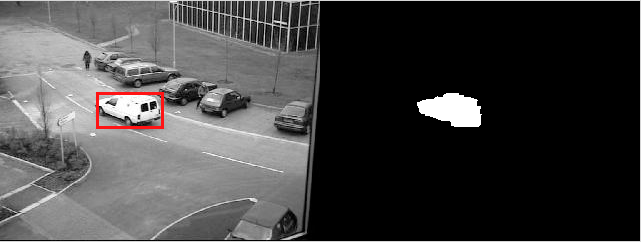
\includegraphics[width=.8\columnwidth]{frameDifferenceCar.png}}\label{fig:frameDifferenceCar}
% \quad
\\\subfloat[Frame difference method on \emph{Highway} sequence]{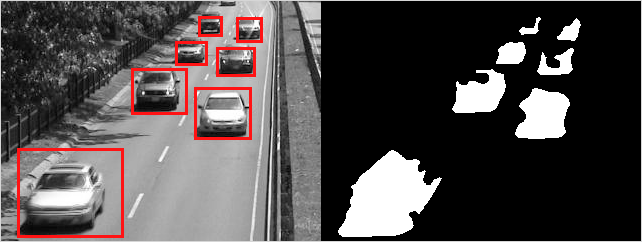
\includegraphics[width=.8\columnwidth]{frameDifferenceHighway.png}\label{fig:frameDifferenceHighway}}
\caption[Frame difference pictures]{Results of frame difference method} % The text in the square bracket is the caption for the list of figures while the text in the curly brackets is the figure caption
\label{fig:frameDifferenceMethod}
\end{figure}

\paragraph{} In order to achieve results on the Figure~\vref{fig:frameDifferenceMethod}, we used many morphological operations as demonstrated in Code Listing~\ref{frameDifferenceCode} 

\matlabscript{frameDifferenceCode}{Morphological operations used for different sequences}


\paragraph{}We also calculated precision, recall and f-score of the results obtained from \emph{Highway} sequence shown in Table ~\ref{table:frameDifferenceScores} .

\begin{table}[h]
\centering
\begin{tabular}{c|c|}
\cline{2-2}
 & \textbf{Score} \\ \hline
\multicolumn{1}{|c|}{\textbf{Precision}} & \%84.17 \\ \hline
\multicolumn{1}{|c|}{\textbf{Recall}} & \%73.92 \\ \hline
\multicolumn{1}{|c|}{\textbf{F-Score}} & \%78.22 \\ \hline
\end{tabular}
\caption{Precision, recall and f-score scores}
\label{table:frameDifferenceScores}
\end{table}

\paragraph{} Overall, this method looks good on the given \emph{Car} and \emph{Highway} sequences. However It will be not enough for more advanced scenarios like high illumination change, cluttered background.

\end{homeworkProblem}

















































%----------------------------------------------------------------------------------------
%	PROBLEM 2
%----------------------------------------------------------------------------------------

\begin{homeworkProblem}
\paragraph{} In problem 2, we asked to use running average Gaussian method. We've given 2 sequence of images. In this method we had mean and sigma images updated continuously. Mean image is used to removed from the current image, and sigma image to get foreground model with some threshold. Sigma image is also updated with learning rate continuously. Like previous method, this method also had problems on initializing and getting stable. After dozen of frames, it becomes more stable and less noisy on \emph{Car} and \emph{Highyway} sequences. Table \vref{table:runningAverageGaussianParameters} on the page \pageref{table:runningAverageGaussianParameters} indicating the parameters of algorithm.

\begin{table}[h]
\centering
\begin{tabular}{|c|c|c|}
\hline
\textbf{Image Sequence} & \textbf{Learning Rate} & \textbf{Threshold} \\ \hline
Car & 0.02 & 3 \\ \hline
Highway & 0.02 & 2.5 \\ \hline
\end{tabular}
\caption{Learning rate and thresholds for sequences}
\label{table:runningAverageGaussianParameters}
\end{table}

\paragraph{} \emph{Highway} sequence has 1700 images. We've asked to use first 470 image training our background and using rest of the images to test and detect cars in the scene. In Figure~\vref{fig:runningAverageGaussianMethod} you can see the results of the method on different image sequences.

\begin{figure}[tbh]
\centering
\subfloat[Running average Gaussian method on \emph{Car} sequence]{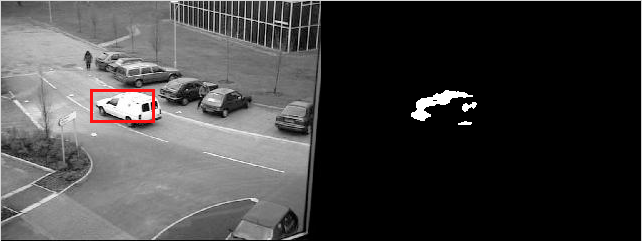
\includegraphics[width=.8\columnwidth]{runningAverageGaussianCar.png}}\label{fig:runningAverageGaussianCar}
% \quad
\\\subfloat[Running average Gaussian method on \emph{Highway} sequence]{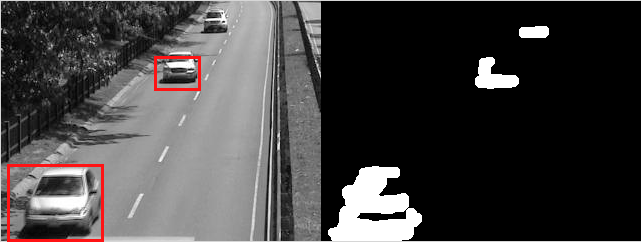
\includegraphics[width=.8\columnwidth]{runningAverageGaussianHighway.png}\label{fig:runningAverageGaussianHighway}}
\caption[Running average Gaussian pictures]{Results of Running average Gaussian method} % The text in the square bracket is the caption for the list of figures while the text in the curly brackets is the figure caption
\label{fig:runningAverageGaussianMethod}
\end{figure}

\paragraph{} In order to achieve results on the Figure~\vref{fig:runningAverageGaussianMethod}, we used many morphological operations as demonstrated in Code Listing~\ref{frameDifferenceCode} .

\matlabscript{runningAverageGaussianCode}{Morphological operations used for different sequences}


\paragraph{}We also calculated precision, recall and f-score of the results obtained from \emph{Highway} sequence shown in Table ~\ref{table:runningAverageGaussianScores} .

\begin{table}[h]
\centering
\begin{tabular}{c|c|}
\cline{2-2}
 & \textbf{Score} \\ \hline
\multicolumn{1}{|c|}{\textbf{Precision}} & \%80.46 \\ \hline
\multicolumn{1}{|c|}{\textbf{Recall}} & \%33.94 \\ \hline
\multicolumn{1}{|c|}{\textbf{F-Score}} & \%44.74 \\ \hline
\end{tabular}
\caption{Precision, recall and f-score scores}
\label{table:runningAverageGaussianScores}
\end{table}

\paragraph{} Overall, this method looks more noisy then the previous method especially on \emph{Highway}. It was challenge for me to detect objects with the method, and unfortunately I didn't able to get stable results. It's also obvious that our recall and f-score is very low. We think we should work on the method to make it more robust against noise and maybe better morphological filtering.


\end{homeworkProblem}

%----------------------------------------------------------------------------------------















































%----------------------------------------------------------------------------------------
%	PROBLEM 3
%----------------------------------------------------------------------------------------

\begin{homeworkProblem}
\paragraph{} In problem 3, Mixture of Gaussians methods was given us, however it was optional to investigate furthermore background subtraction methods. So we implemented it to see and experiment. We only tested the method on \emph{Car} sequence. So no training and testing is done for \emph{Highway} sequence. We think it was most the complicated method among others. It was using the multiple Gaussian distribution to model each pixel. We used 3 Gaussian distribution on testing the method on \emph{Car} sequence. It was also the slowest method among others, however result was more better than running average Gaussian method.

\begin{figure}[tbh]
\centering
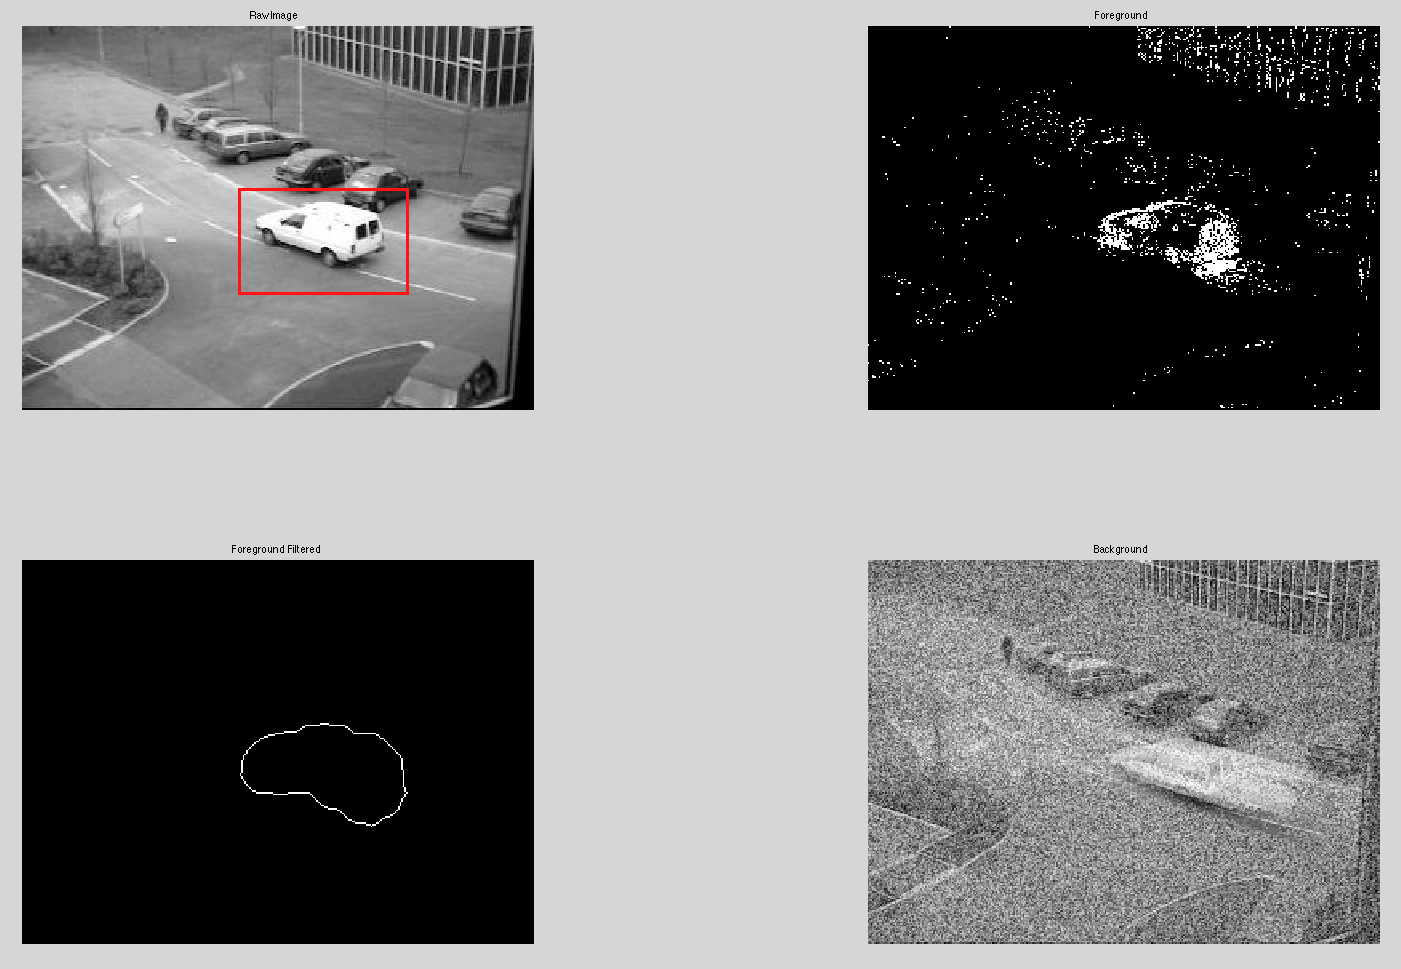
\includegraphics[width=1\columnwidth]{mixtureOfGaussiansCar.png}\label{fig:mixtureOfGaussiansCar}
\caption{Result of mixture of Gaussians method on \emph{Car} sequence}
\label{fig:mixtureOfGaussiansMethodasd}
\end{figure}
\paragraph{} In order to achieve results on the Figure~\ref{fig:mixtureOfGaussiansMethodasd}, we used many morphological operations as demonstrated in Code Listing~\ref{mixtureOfGaussiansCode} .

\matlabscript{mixtureOfGaussiansCode}{Morphological operations used for \emph{Car} sequence}

\paragraph{} Overall, it was complex method to implement. It was running slow with large number of Gaussian distributions. In conclusion, its stable method and producing less noisy foreground model. It's more efficient implementation then current one is left as a future work :)

\end{homeworkProblem}

%----------------------------------------------------------------------------------------













































%----------------------------------------------------------------------------------------
%	PROBLEM 4
%----------------------------------------------------------------------------------------

\begin{homeworkProblem}
\paragraph{} In problem 4, we asked to use Eigen Background method. We've given 2 sequence of images. In this method, we first calculated mean image for each sequence from each image. Then we normalized our images by subtracting mean image from them. Then applied PCA via SVD by finding some subspace that spanning our images. This method we think so produced stable results then others on \emph{Car} and \emph{Highway} sequences. We used our subspace size as number of images divided by number of images in sequence to fulfill $k \textless\textless N$ constraint.

\paragraph{} \emph{Highway} sequence has 1700 images. We've asked to use first 470 image training our background and using rest of the images to test and detect cars in the scene. In Figure~\vref{fig:eigenBackgroundMethod} you can see the results of the method on difference image sequences.

\begin{figure}[tbh]
\centering
\subfloat[Eigen Background method on \emph{Car} sequence]{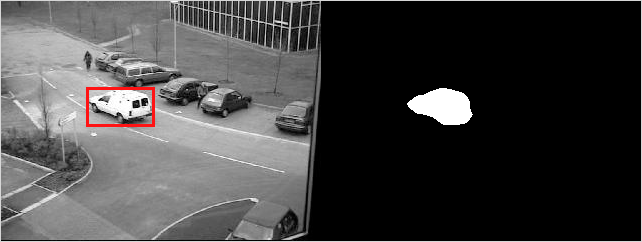
\includegraphics[width=.8\columnwidth]{eigenBackgroundCar.png}}\label{fig:eigenBackgroundCar}
% \quad
\\\subfloat[Eigen Background method on \emph{Highway} sequence]{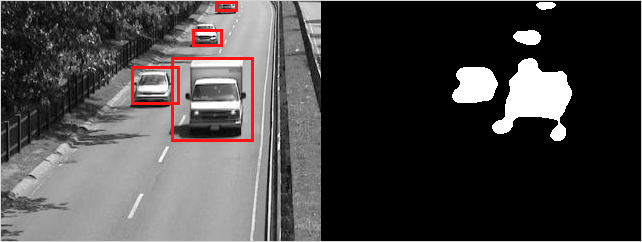
\includegraphics[width=.8\columnwidth]{eigenBackgroundHighway.png}\label{fig:eigenBackgroundHighway}}
\caption[Eigen Background pictures]{Results of Eigen Background method} % The text in the square bracket is the caption for the list of figures while the text in the curly brackets is the figure caption
\label{fig:eigenBackgroundMethod}
\end{figure}

\paragraph{} In order to achieve results on the Figure~\vref{fig:eigenBackgroundMethod}, we used many morphological operations as demonstrated in Code Listing~\ref{eigenBackgroundCode} .

\matlabscript{eigenBackgroundCode}{Morphological operations used for different sequences}


\paragraph{}We also calculated precision, recall and f-score of the results obtained from \emph{Highway} sequence shown in Table ~\ref{table:eigenBackgroundScores} .

\begin{table}[h]
\centering
\begin{tabular}{c|c|}
\cline{2-2}
 & \textbf{Score} \\ \hline
\multicolumn{1}{|c|}{\textbf{Precision}} & \%95.71 \\ \hline
\multicolumn{1}{|c|}{\textbf{Recall}} & \%79.28 \\ \hline
\multicolumn{1}{|c|}{\textbf{F-Score}} & \%85.98 \\ \hline
\end{tabular}
\caption{Precision, recall and f-score scores}
\label{table:eigenBackgroundScores}
\end{table}

\paragraph{} In conclusion, the Eigen Background method looks very stable and fast among others on \emph{Car} and \emph{Highway} sequences. It produce nice results with less noise. We think its also easy to implement. Whereas when the data-set is increasing by more images in sequences, it's getting hard to manage matrix operations, i.e., using SVD, where we had to use economy mode of it. As a result, it has the highest F-Score, it was easy to implement and fast. We would prefer this method to be used in our further works.

\end{homeworkProblem}

%----------------------------------------------------------------------------------------


\section{Conclusion}

In this lab, we reviewed Frame differencing, Running average Gaussian, Mixture of Gaussians and Eigen Background. Eigen Background and Frame difference methods produced nice results while tracking the objects. However all methods had problems with backgrounds like in \emph{Highway}, where there was trees, very small camera vibration. We think these methods alone cannot overcome the very cluttered backgrounds nor camera motion or very high illumination change.  





\end{document}